%% fig_bypass.tex   (generated by make_frontier.py; do not edit by hand)
%% The audit of the bypass mechanisms for the Mumford target.
\documentclass[tikz,border=8pt]{standalone}
\usepackage{amsmath,amssymb}
\usetikzlibrary{arrows.meta,calc,decorations.pathreplacing}
%% palette.tex -- shared colour definitions for the figures
\definecolor{PInk}{RGB}{26,32,44}
\definecolor{PBlue}{RGB}{37,82,139}
\definecolor{PTeal}{RGB}{23,127,125}
\definecolor{POchre}{RGB}{193,138,44}
\definecolor{PClay}{RGB}{178,74,58}
\definecolor{PSlate}{RGB}{108,122,137}
\definecolor{PViolet}{RGB}{110,86,150}
\definecolor{WBlue}{RGB}{223,234,246}
\definecolor{WTeal}{RGB}{220,238,236}
\definecolor{WOchre}{RGB}{250,240,218}
\definecolor{WClay}{RGB}{247,229,224}
\definecolor{WSlate}{RGB}{238,241,244}
\definecolor{PMag}{RGB}{158,58,110}
\definecolor{PGrass}{RGB}{62,124,66}
\definecolor{PAmber}{RGB}{214,112,38}
\definecolor{PIndigo}{RGB}{58,64,140}
\definecolor{PRule}{RGB}{176,186,197}

%% shared macros so the standalone figures match the paper
\providecommand{\QQ}{\mathbb{Q}}
\providecommand{\ZZ}{\mathbb{Z}}
\providecommand{\RR}{\mathbb{R}}
\providecommand{\CC}{\mathbb{C}}
\providecommand{\PP}{\mathbb{P}}
\providecommand{\Kx}{K^{\times}}
\providecommand{\HW}{W}
\providecommand{\Nm}{\mathrm{N}}
\providecommand{\Hdg}{\mathrm{Hdg}}
\providecommand{\NS}{\mathrm{NS}}
\providecommand{\cA}{\mathcal{A}}
\providecommand{\cD}{\mathcal{D}}
\providecommand{\cF}{\mathcal{F}}
\providecommand{\cP}{\mathcal{P}}
\providecommand{\cO}{\mathcal{O}}
\providecommand{\cQ}{\mathcal{Q}}
\providecommand{\bbar}[1]{\overline{#1}}
\providecommand{\ch}{\operatorname{ch}}
\providecommand{\End}{\mathrm{End}}

\newcommand{\hcimp}{\,\textcolor{PIndigo}{\tiny$\Leftarrow\mathbf{HC}$}}
\begin{document}
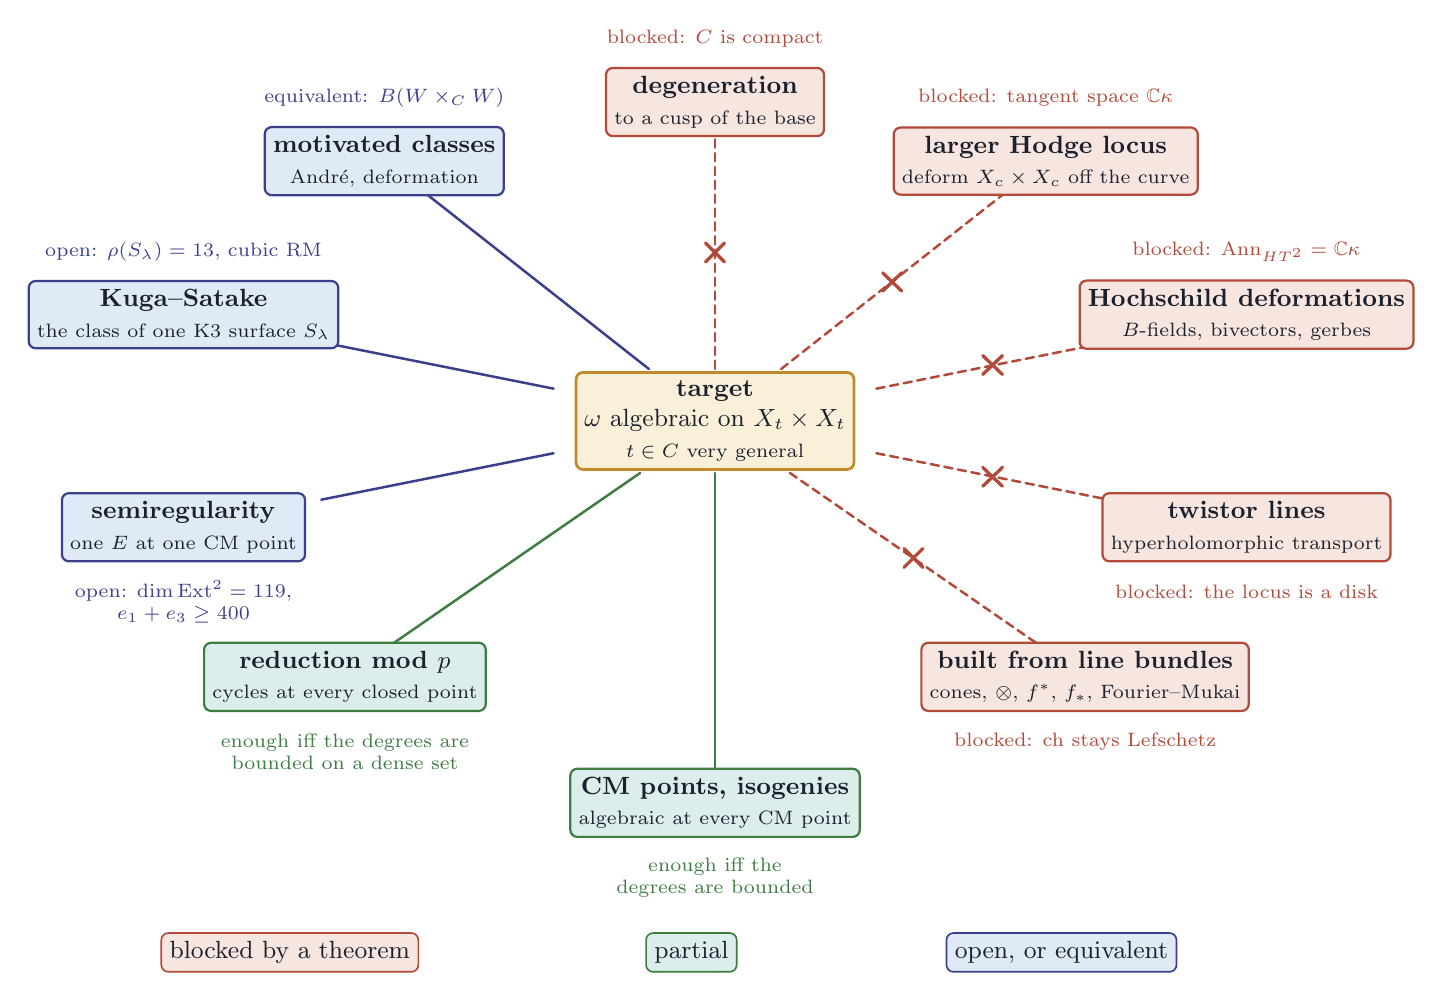
\begin{tikzpicture}[x=1cm,y=1cm,line join=round,line cap=round,
  font=\small,text=PInk]
  \node[draw=POchre,fill=WOchre,rounded corners=2.5pt,inner sep=3pt,line width=1.00pt,align=center] at (0.00,0.00) {\textbf{target}\\$\omega$ algebraic on $X_{t}\times X_{t}$\\{\scriptsize $t\in C$ very general}};
  \draw[PClay,line width=0.9pt,dash pattern=on 3pt off 2pt] (0.00,0.66) -- (0.00,3.62);
  \draw[PClay,line width=1.2pt] (-0.12,2.02) -- (0.12,2.26) (-0.12,2.26) -- (0.12,2.02);
  \node[draw=PClay,fill=WClay,rounded corners=2.5pt,inner sep=3pt,line width=0.80pt,align=center] at (0.00,4.05) {\textbf{degeneration}\\{\scriptsize to a cusp of the base}};
  \node[text=PClay,inner sep=1pt,align=center,font=\scriptsize] at (0.00,4.85) {blocked: $C$ is compact};
  \draw[PClay,line width=0.9pt,dash pattern=on 3pt off 2pt] (0.84,0.66) -- (3.65,2.87);
  \draw[PClay,line width=1.2pt] (2.13,1.65) -- (2.37,1.88) (2.13,1.88) -- (2.37,1.65);
  \node[draw=PClay,fill=WClay,rounded corners=2.5pt,inner sep=3pt,line width=0.80pt,align=center] at (4.20,3.30) {\textbf{larger Hodge locus}\\{\scriptsize deform $X_{c}\times X_{c}$ off the curve}};
  \node[text=PClay,inner sep=1pt,align=center,font=\scriptsize] at (4.20,4.10) {blocked: tangent space $\CC\kappa$};
  \draw[PClay,line width=0.9pt,dash pattern=on 3pt off 2pt] (2.05,0.41) -- (5.00,1.00);
  \draw[PClay,line width=1.2pt] (3.40,0.59) -- (3.65,0.83) (3.40,0.83) -- (3.65,0.59);
  \node[draw=PClay,fill=WClay,rounded corners=2.5pt,inner sep=3pt,line width=0.80pt,align=center] at (6.75,1.35) {\textbf{Hochschild deformations}\\{\scriptsize $B$-fields, bivectors, gerbes}};
  \node[text=PClay,inner sep=1pt,align=center,font=\scriptsize] at (6.75,2.15) {blocked: $\mathrm{Ann}_{HT^{2}}=\CC\kappa$};
  \draw[PClay,line width=0.9pt,dash pattern=on 3pt off 2pt] (2.05,-0.41) -- (5.00,-1.00);
  \draw[PClay,line width=1.2pt] (3.40,-0.83) -- (3.65,-0.59) (3.40,-0.59) -- (3.65,-0.83);
  \node[draw=PClay,fill=WClay,rounded corners=2.5pt,inner sep=3pt,line width=0.80pt,align=center] at (6.75,-1.35) {\textbf{twistor lines}\\{\scriptsize hyperholomorphic transport}};
  \node[text=PClay,inner sep=1pt,align=center,font=\scriptsize] at (6.75,-2.17) {blocked: the locus is a disk};
  \draw[PClay,line width=0.9pt,dash pattern=on 3pt off 2pt] (0.95,-0.66) -- (4.08,-2.82);
  \draw[PClay,line width=1.2pt] (2.40,-1.86) -- (2.64,-1.62) (2.40,-1.62) -- (2.64,-1.86);
  \node[draw=PClay,fill=WClay,rounded corners=2.5pt,inner sep=3pt,line width=0.80pt,align=center] at (4.70,-3.25) {\textbf{built from line bundles}\\{\scriptsize cones, $\otimes$, $f^{*}$, $f_{*}$, Fourier--Mukai}};
  \node[text=PClay,inner sep=1pt,align=center,font=\scriptsize] at (4.70,-4.07) {blocked: $\mathrm{ch}$ stays Lefschetz};
  \draw[PGrass,line width=0.9pt] (0.00,-0.66) -- (0.00,-4.42);
  \node[draw=PGrass,fill=WTeal,rounded corners=2.5pt,inner sep=3pt,line width=0.80pt,align=center] at (0.00,-4.85) {\textbf{CM points, isogenies}\\{\scriptsize algebraic at every CM point}};
  \node[text=PGrass,inner sep=1pt,align=center,font=\scriptsize] at (0.00,-5.80) {enough iff the\\degrees are bounded};
  \draw[PGrass,line width=0.9pt] (-0.95,-0.66) -- (-4.08,-2.82);
  \node[draw=PGrass,fill=WTeal,rounded corners=2.5pt,inner sep=3pt,line width=0.80pt,align=center] at (-4.70,-3.25) {\textbf{reduction mod $p$}\\{\scriptsize cycles at every closed point}};
  \node[text=PGrass,inner sep=1pt,align=center,font=\scriptsize] at (-4.70,-4.20) {enough iff the degrees are\\bounded on a dense set};
  \draw[PIndigo,line width=0.9pt] (-2.05,-0.41) -- (-5.00,-1.00);
  \node[draw=PIndigo,fill=WBlue,rounded corners=2.5pt,inner sep=3pt,line width=0.80pt,align=center] at (-6.75,-1.35) {\textbf{semiregularity}\\{\scriptsize one $E$ at one CM point}};
  \node[text=PIndigo,inner sep=1pt,align=center,font=\scriptsize] at (-6.75,-2.30) {open: $\dim\mathrm{Ext}^{2}=119$,\\$e_{1}+e_{3}\ge400$};
  \draw[PIndigo,line width=0.9pt] (-2.05,0.41) -- (-5.00,1.00);
  \node[draw=PIndigo,fill=WBlue,rounded corners=2.5pt,inner sep=3pt,line width=0.80pt,align=center] at (-6.75,1.35) {\textbf{Kuga--Satake}\\{\scriptsize the class of one K3 surface $S_{\lambda}$}};
  \node[text=PIndigo,inner sep=1pt,align=center,font=\scriptsize] at (-6.75,2.15) {open: $\rho(S_{\lambda})=13$, cubic RM};
  \draw[PIndigo,line width=0.9pt] (-0.84,0.66) -- (-3.65,2.87);
  \node[draw=PIndigo,fill=WBlue,rounded corners=2.5pt,inner sep=3pt,line width=0.80pt,align=center] at (-4.20,3.30) {\textbf{motivated classes}\\{\scriptsize Andr\'e, deformation}};
  \node[text=PIndigo,inner sep=1pt,align=center,font=\scriptsize] at (-4.20,4.10) {equivalent: $B(W\times_{C}W)$};
  \node[draw=PClay,fill=WClay,rounded corners=2.5pt,inner sep=3pt,line width=0.60pt,align=center] at (-5.40,-6.75) {blocked by a theorem};
  \node[draw=PGrass,fill=WTeal,rounded corners=2.5pt,inner sep=3pt,line width=0.60pt,align=center] at (-0.30,-6.75) {partial};
  \node[draw=PIndigo,fill=WBlue,rounded corners=2.5pt,inner sep=3pt,line width=0.60pt,align=center] at (4.40,-6.75) {open, or equivalent};
\end{tikzpicture}
\end{document}
